\chapter{Installing and Running GenOpt}
\label{sec:InsAndRunGen}
\section{System Requirements}
To run GenOpt and the GenOpt installation program, a Java \javaversion runtime environment is required.
GenOpt should run on any operating system that can run Java applications.

\section{Installing and uninstalling GenOpt}
To install GenOpt, download the installation program
{\tt genopt-install.jar} from
\url{http://SimulationResearch.lbl.gov/GO}.
Then, either double-click on the file {\tt genopt-install.jar}\footnote{Depending on your Java installation, the file extension {\tt jar} may not be associated with Java. In this situation, please consult the instructions of your operating system for how to associate file extensions with programs.}
or open a command shell, change to the directory that contains {\tt genopt-install.jar} and type
\begin{lstlisting}
  java -jar genopt-install.jar
\end{lstlisting}
No environment variables need to be set to run GenOpt. (This is new since GenOpt~2.1.0.)

Note that Windows~7, depending on the permission of the user account, may not allow the GenOpt installation program to install GenOpt in {\tt C:\textbackslash Program Files}. In this situation, GenOpt can be installed in another programs, and then moved to {\tt C:\textbackslash Program Files}.\\

To uninstall GenOpt, delete the directory in which GenOpt was installed.

% ----------------------------------------------------------
\section{Running GenOpt}
\subsection{Running GenOpt from the file explorer}
To run GenOpt from the file explorer,
double-click on the file {\tt genopt.jar}.$^1$
This will start the graphical user interface. 
From the graphical user interface, select {\tt File},
{\tt Start...} and select a GenOpt initialization file.

\subsection{Running GenOpt from the command line}
GenOpt can also be run as a console application, either with or without the graphical user interface. 
To run GenOpt as a console application with the graphical user interface, open a shell, change to the directory that contains
{\tt genopt.jar} and type
\begin{lstlisting}
  java -jar genopt.jar [initializationFile]
\end{lstlisting}
where {\tt [initializationFile]} is an optional argument that can be
replaced with the GenOpt initialization file (see example below).
To start GenOpt without the graphical user interface, type
\begin{lstlisting}
  java -classpath genopt.jar genopt.GenOpt [initializationFile]
\end{lstlisting}
\newpage
For instance, to run the example file provided with GenOpt that minimizes a quadratic function using the Hooke-Jeeves algorithm, 
type on Mac OS~X
\begin{lstlisting}
  java -jar genopt.jar example/quad/GPSHookeJeeves/optMacOSX.ini
\end{lstlisting}
on Linux
\begin{lstlisting}
  java -jar genopt.jar example/quad/GPSHookeJeeves/optLinux.ini
\end{lstlisting}
and on Windows 
\begin{lstlisting}
  java -jar genopt.jar example\quad\GPSHookeJeeves\optWinXP.ini
\end{lstlisting}
This should produce the window shown in Fig.~\ref{fig:wingenoptGPSHJ}.

\begin{figure}
\centering
\epsfig{file=img/wingenopt.eps, width=\headwidth}
\caption{Output of GenOpt on Mac OS X for the example file in the directory {\tt example/quad/GPSHookeJeeves}.}
\label{fig:wingenoptGPSHJ}
\end{figure}
